\section{Collaborative Filtering Recommender System: User-Based }
In this chapter, we will demonstrate the implementation of a user-based recommender system.

\textbf{\textit{Dataset}}. In this system, we adopt the dataset called MovieLen \cite{movielens}. MovieLen contains 100,000 ratings and 3,600 tag applications applied to 9,000 movies by 600 users.

\textbf{\textit{Implementation}}. By \textit{pandas} library, we read movies and ratings into the data frame. The format of both movie and rating data frames is shown in Figure 4.13.
    \begin{figure}[htbp]
\centering
\subfigure[movies data-frame]{
\begin{minipage}[t]{0.5\linewidth}
\centering
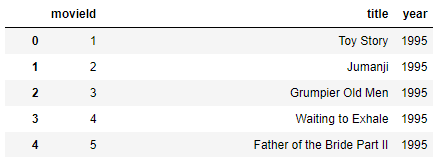
\includegraphics[scale=0.6]{figure/usercf1.png}
%\caption{fig1}
\end{minipage}%
}%
\subfigure[ratings data-frame]{
\begin{minipage}[t]{0.5\linewidth}
\centering
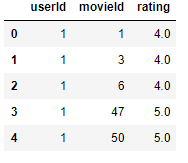
\includegraphics[scale=0.7]{figure/cf2.png}
%\caption{fig2}
\end{minipage}%
}%
\centering
\caption{Format of data frame}
\end{figure} 

According to the process for creating memory-based collaborative filtering, the next step is to identify a target user who will be recommended.

\textbf{\textit{Identify a target user}}. We define a target user and their rating in the way shown in the frame below. As in the image shown in Figure 4.14, the target user data frame involved the movie title with its ID and the target user’s rating. 
\begin{framed} 
\textbf{Target user input}\\
\rule{\textwidth}{0.1mm}
targetUserInput = [\\
{'title':'Grumpier Old Men', 'rating':4},\\
{'title':'Get Shorty', 'rating':2.5},\\
{'title':'Pulp Fiction', 'rating':3},\\
{'title':"Heat", 'rating':3.5},\\
{'title':'Toy Story', 'rating':5}\\
         ] \\
targetUserMovies = pd.DataFrame(targetUserInput)\\
targetUserMovies\\
\end{framed} 

\begin{figure}[htbp]
\centering
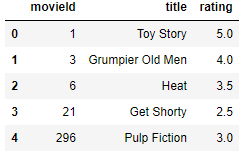
\includegraphics[scale =1]{figure/targetcf1.png}
\caption{Target user data frame}
\end{figure}

\textbf{\textit{Find similar user}}. With the movie ID in the target user input, we can now figure out the users who have seen and rated the movie, which is the same as the target user input. Then, according to the user ID, we group up the rows of the similar user sets. We sort these groups, with the rule that the group with more number of the movies watched or rated the same as the target user will be given a higher priority. With the information contained in Figure 4.15, the groups with user IDs 32, 91, and 414 are the groups that have the top 3 highest numbers of movies watched or rated the same as the target user.


\begin{figure}[htbp]
\centering
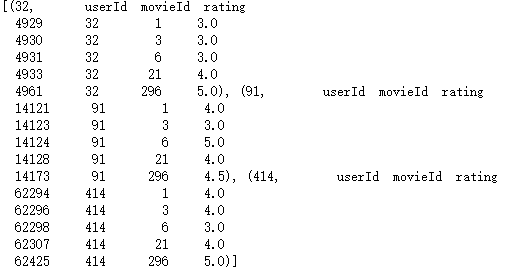
\includegraphics[scale =0.7]{figure/targecf2.png}
\caption{Top three similar groups}
\end{figure}

\textbf{\textit{Calculate the similarity}}. In this step, we are going to compare all groups with the target user to figure out the most similar one by calculating the similarity by formula. As mentioned in the methodology chapter, there exist many formulae to calculate the similarity, but in this system, \textit{Pearson Correlation Coefficient} is adopted, and it can be represented as :
\begin{equation}
    \operatorname{sim}(i, j)=\frac{\sum_{p \in P}\left(R_{i, p}-\bar{R}_{i}\right)\left(R_{j, p}-\bar{R}_{j}\right)}{\sqrt{\sum_{p \in P}\left(R_{i, p}-\bar{R}_{i}\right)^{2}} \sqrt{\sum_{p \in P}\left(R_{j, p}-\bar{R}_{j}\right)^{2}}}
\end{equation}
where $R_{i, p}$ denote the rating of the user $i$ on movie $p$ and $\bar{R}_{i}$ represents the average rating of all movies by the user $i$. Similarly, $R_{j, p}$ denote the rating of the target user $j$ on movie $p$ and $\bar{R}_{j}$ represents the average rating of all movies by the target user $j$. Also, $P$ represents the set of all movies.

\begin{figure}
    \centering
    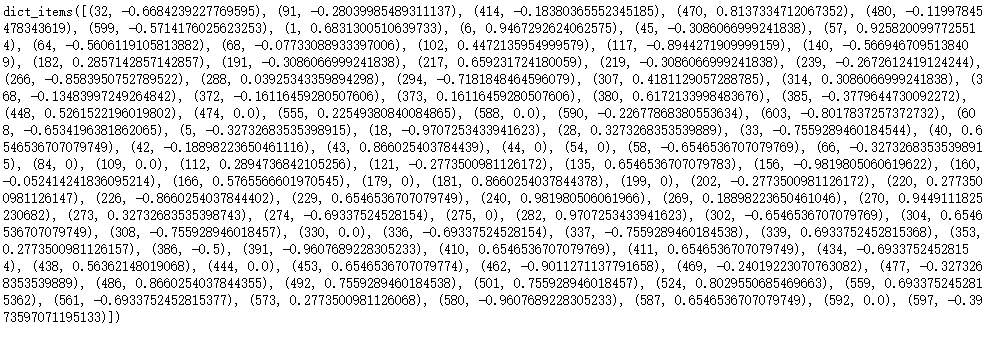
\includegraphics[scale=0.6]{figure/cf7.png}
    \caption{Similarity value of all similar users to the target user}
\end{figure}
After calculating the similarity, we can list out the similarity of all similar users to the target user, as shown in Figure 4.16.
\begin{figure}
    \centering
    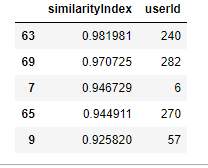
\includegraphics[scale=1]{figure/taegetcf3.png}
    \caption{Top 5 similar users }
\end{figure}
As Figure 4.17 shows, by sorting the similar users by similarity, the user with ID 240 is the most similar user with the target user, for whom the similarity is 0.981981.

\begin{figure}[htbp]
\centering
\subfigure[Weighted rating]{
\begin{minipage}[t]{0.33\linewidth}
\centering
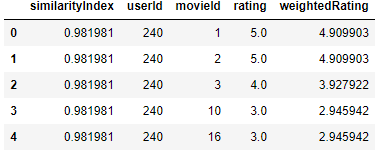
\includegraphics[scale=0.6]{figure/tar4.png}
%\caption{fig1}
\end{minipage}%
}%
\subfigure[Sum of the weighted rating]{
\begin{minipage}[t]{0.33\linewidth}
\centering
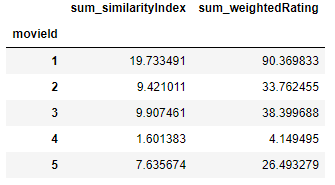
\includegraphics[scale=0.6]{figure/tar5.png}
%\caption{fig2}
\end{minipage}%
}%
\subfigure[Weighted average score]{
\begin{minipage}[t]{0.33\linewidth}
\centering
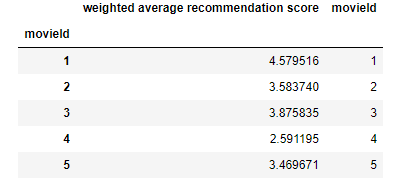
\includegraphics[scale=0.6]{figure/tar6.png}
%\caption{fig2}
\end{minipage}
}%
\centering
\caption{Calculate the score for recommendation (5 out of 9000 movies)}
\end{figure}
By the method of user-based collaborative filtering, we multiply the similar user’s rating by the similarity to get the weighted rating. As shown in Figure 4.18 (a), the intuition here is that the higher the similarity with the target user, the higher the weight of the target user's prediction score. Figure 4.18 (b) demonstrates the result of the sum of weighted ratings and the sum of similarity. Finally, in Figure 4.18 (c), by dividing the sum of weighted ratings by the sum of similarity, we can get the predicted weighted average recommendation score of what the target users probably rate the movie.

\textbf{\textit{Recommendation}}. For the recommendation, based on the above steps, first, sort the movies by average recommendation score, which is shown in Figure 4.19 (a). Then, by the movie ID in the sort list, we can get the top 10 movies with titles recommended by the user-based collaborative filtering system to the target user, as shown in Figure 4.19 (b).

 \begin{figure}[htbp]
\centering
\subfigure[Sorted by average recommendation score]{
\begin{minipage}[t]{0.5\linewidth}
\centering
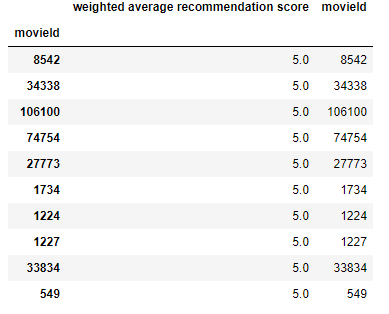
\includegraphics[scale=0.7]{figure/tar7.png}
%\caption{fig1}
\end{minipage}%
}%
\subfigure[recommend movies]{
\begin{minipage}[t]{0.5\linewidth}
\centering
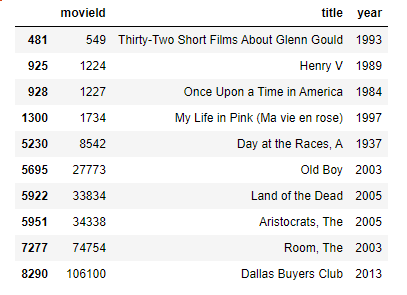
\includegraphics[scale=0.7]{figure/tar8.png}
%\caption{fig2}
\end{minipage}%
}%
\centering
\caption{Top 10 movies recommend by user-based system }
\end{figure}